Let 
\begin{align}
  x\brak{t}&=\cos{\brak{20k\pi t}}
  &= \cos{\cbrak{2\pi (10k) t}}
  \\
  \implies B_x &= 10 kHz
\end{align}
where $B_x$ is the bandwidth of $x(t)$.  Then 
\begin{align}
    y\brak{t}&= \cos{\brak{30k\pi t}}+\cos{\brak{10k\pi t}}\\
    \implies B_y &= \frac{30}{2} 
    &= 15 kHz
\end{align}
Thus, the Nyquist rate is 
\begin{align}
B &= 2 B_y\\
    &= 30 kHz
\end{align}
Figs.  \ref{ec/2021/4/1}- \ref{ec/2021/4/5} show the sampling theorem in action.  Fig. \ref{ec/2021/4/5} shows
how the violation of the the Nyquist criterion results in distortion during reconstruction.
%
\begin{figure}[!h]
 \centering
 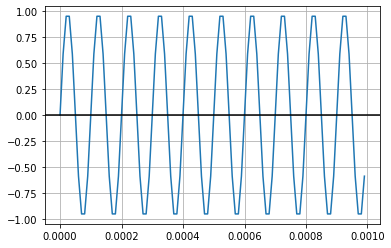
\includegraphics[width=\columnwidth]{solutions/ec/2021/4/figs/x.png}
 \caption{$x\brak{t}$:Sinusoidal signal with freq=10kHz}
 \label{ec/2021/4/1}
\end{figure}
\begin{figure}[!h]
 \centering
 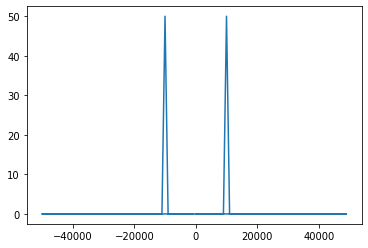
\includegraphics[width=\columnwidth]{solutions/ec/2021/4/figs/xf.png}
 \caption{DFT of $x\brak{t}$. $Bandwidth=10000$}
 \label{ec/2021/4/2}
 \end{figure}
\begin{figure}[!h]
 \centering
 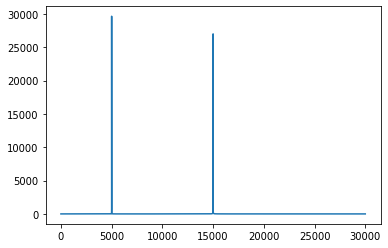
\includegraphics[width=\columnwidth]{solutions/ec/2021/4/figs/four_y.png}
 \caption{DFT of $y\brak{t}$.$Bandwidth=15000$}
 \label{ec/2021/4/3}
 \end{figure}
\begin{figure}[!h]
 \centering
 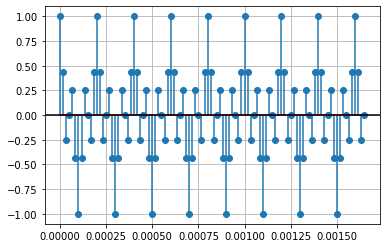
\includegraphics[width=\columnwidth]{solutions/ec/2021/4/figs/stem_y.png}
 \caption{stem plot of $y\brak{t}$ sampled at 60kHz}
 \label{ec/2021/4/4}
 \end{figure}
\begin{figure}[!h]
 \centering
 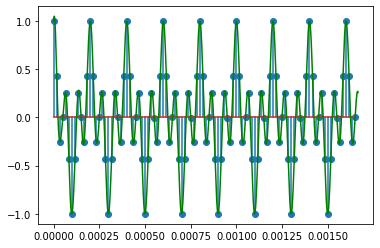
\includegraphics[width=\columnwidth]{solutions/ec/2021/4/figs/interpolation.png}
 \caption{Shannon interpolation of $y\brak{t}$}
 \label{ec/2021/4/5}
 \end{figure}


